\documentclass[10pt]{beamer}
\usefonttheme{professionalfonts,serif}
\def\newblock{\hskip .11em plus .33em minus .07em}
\usepackage[numbers,sort]{natbib}
\renewcommand{\rmdefault}{psbx}
\usepackage[utf8]{inputenc}
\usepackage[T1]{fontenc}
\usepackage{textcomp}
\usepackage{eulervm}

\usetheme{default}           % tips from David Blei
\useinnertheme{circles}
\useoutertheme{infolines}
\setbeamertemplate{headline}{}
\setbeamertemplate{navigation symbols}{}
\setbeamerfont{itemize/enumerate subbody}{size=\normalsize}
\setbeamerfont{itemize/enumerate subsubbody}{size=\normalsize}
\usecolortheme{seahorse}
\setbeamersize{text margin left=2mm,text margin right=2mm}

\graphicspath{{../../figures/}}

\definecolor{mypine}{rgb}{0.05,0.45,0.05}
\definecolor{mycyan}{rgb}{0.0,0.9,0.9}
\newcommand{\Red}{\textcolor{red}}
\newcommand{\Blue}{\textcolor{blue}}
\newcommand{\Green}{\textcolor{mypine}}
\newcommand{\PineGreen}{\textcolor{mypine}}
\newcommand{\Magenta}{\textcolor{magenta}}
\newcommand{\Cyan}{\textcolor{mycyan}}

\newcommand{\N}{\mathcal{N}}
\newcommand{\R}{\mathbb{R}}
\newcommand{\T}{{\scriptsize^{\top}}}
\newcommand{\D}{\mathcal{D}}
\newcommand{\F}{\mathcal{F}}
\newcommand{\E}{\mathbb{E}}
\newcommand{\V}{\mathbb{V}}
\newcommand{\M}{\mathcal{M}}
\newcommand{\KL}{\mathcal{KL}}
\newcommand{\cut}[1]{}
\newcommand{\trace}{\operatorname{trace}}

\newcommand{\bmu}{{\boldsymbol{\mu}}}
\newcommand{\btheta}{\boldsymbol{\theta}}
\newcommand{\bepsilon}{\boldsymbol{\epsilon}}
\newcommand{\balpha}{\boldsymbol{\alpha}}
\newcommand{\bbeta}{\boldsymbol{\beta}}
\newcommand{\bphi}{\boldsymbol{\phi}}
\newcommand{\bPhi}{\boldsymbol{\Phi}}
\newcommand{\bSigma}{\boldsymbol{\Sigma}}
\newcommand{\bpi}{\boldsymbol{\pi}}
\newcommand{\blambda}{\boldsymbol{\lambda}}

\newcommand{\argmax}{\operatorname{argmax}}
\newcommand{\argmin}{\operatorname{argmin}}
\newcommand{\ci}{{\bot\negthickspace\negthickspace\bot}} % conditional indep.
\newcommand{\neigh}{\operatorname{ne}}
\newcommand{\vectr}[2]{  \left[ \!\!\begin{array}{c} #1 \\
      #2 \end{array} \!\!\right]}
\newcommand{\deff}{\stackrel{\mathrm{def}}{=}}
\newcommand{\deldel}[2]{\frac{\partial #1}{\partial #2}}

\newcommand{\maketilde}{\raisebox{0.4ex}{\tiny $\sim$}}
\newcommand{\bfa}{\mathbf a}
\newcommand{\bfb}{\mathbf b}
\newcommand{\bfe}{\mathbf e}
\newcommand{\bff}{\mathbf f}
\newcommand{\bfk}{\mathbf k}
\newcommand{\bfm}{\mathbf m}
\newcommand{\bfn}{\mathbf n}
\newcommand{\bfp}{\mathbf{p}}
\newcommand{\bfs}{\mathbf s}
\newcommand{\bfu}{\mathbf u}
\newcommand{\bfx}{\mathbf x}
\newcommand{\bfy}{\mathbf y}
\newcommand{\bft}{\mathbf t}
\newcommand{\bfv}{\mathbf v}
\newcommand{\bfw}{\mathbf w}
\newcommand{\bfA}{\mathbf A}
\newcommand{\bfI}{\mathbf I}
\newcommand{\bfK}{\mathbf K}


\title{Distributions over parameters and functions}
\author{Carl Edward Rasmussen}
\date{October 13th, 2016}

\begin{document}

\begin{frame}
\titlepage
\end{frame}

\begin{frame}
\frametitle{Key concepts}

\begin{itemize}
\item In a parametric model, the model is represented using \Red{parameters}
\item a distribution over parameters implies a distribution over functions
\item In Bayesian inference, we marginalize over parameters to make predictions
\item Question: could we work directly in the space of functions?
\end{itemize}
\end{frame}


\begin{frame}
\frametitle{Priors on parameters induce priors on functions}

A model $\mathcal{M}$ is the choice of a \Red{model structure} and of \Blue{parameter values}.  
%
\[
f_\bfw(x)\; =\; \sum_{m=0}^{\Red{M}} \Blue{w_m}\,\Red{\phi_m(x)}
\]
%
The prior $p(\bfw|\mathcal{M})$ determines what \Blue{functions} this model can generate. Example:
\begin{itemize}
\item Imagine we choose $M=17$, and $p(w_m)=\N(w_m;\;0, \sigma_\bfw^2)$. 
\item We have actually defined a \Blue{prior distribution over functions $p(\bff|\mathcal{M})$}. 
\end{itemize} \vspace*{-1.5ex}

\parbox{0.49\textwidth}{
This figure is generated as follows: 
\begin{itemize}
\item Use polynomial basis functions, $\phi_m(x)=x^m$. 
\item Define a uniform grid of $n=100$ values in $x$ from $[-1.5, 2]$. 
\item Generate matrix $\bPhi$ for $M=17$. 
%\texttt{Phi = repmat(x,1,M+1).\^{}repmat(0:M,N,1);}
\item Draw $w_m\sim{\cal N}(0,1)$. 
\item Compute and plot $\bff=\bPhi_{n\times 18}\,\bfw$. 
\end{itemize}
}
\parbox{0.45\textwidth}{
\centerline{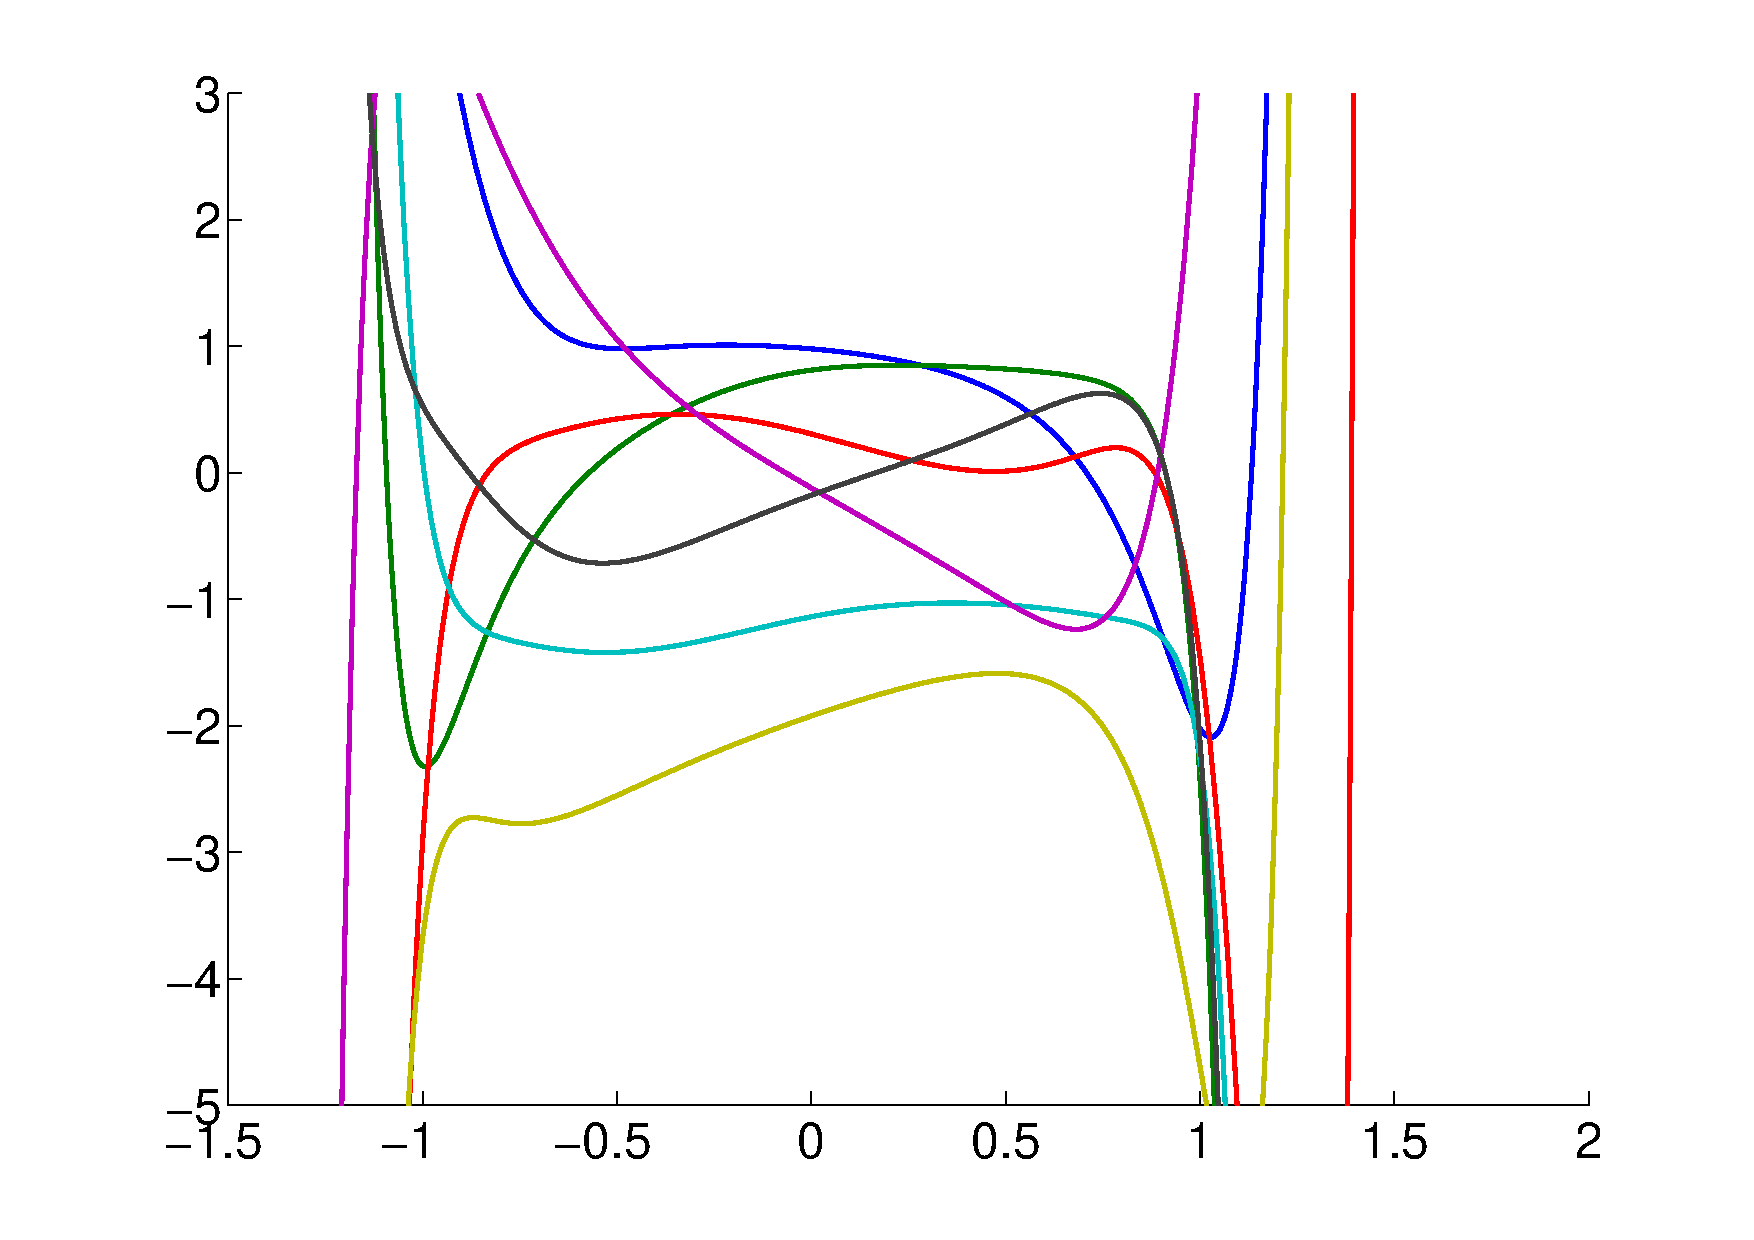
\includegraphics[width=0.5\textwidth]{random_polynomials_degree17.pdf}}
}
\end{frame}


\begin{frame}
\frametitle{Nuissance parameters and distributions over functions}

We've seen that distributions over parameters induce distributions
over functions.\\[1ex]

We've set up a scheme where we
\begin{itemize}
\item first set up a model in terms a parameters
\item then marginalize out the parameters
\end{itemize}
Typically, we're not really interested in \Red{parameters}, we're interested
in \Blue{predictions}.\\[1ex]

The parameters are a \Red{nuissance}.\\[1ex]

Could we possibly work \Blue{directly} in the space of functions?
\begin{itemize}
\item simpler inference
\item better understading of the distributions over functions
\end{itemize}
\end{frame}


\begin{frame}
\frametitle{Posterior probability of a function}

Given the \Blue{prior}  functions \Blue{$p(\bff)$} how can we make predictions?
\begin{itemize}
\item Of all functions generated from the prior, keep those that fit the data.
\item The notion of closeness to the data is given by the \Red{likelihood $p(\bfy|\bff)$}.
\item We are really interested in the posterior distribution over functions:
%
\[
\Green{p(\bff|\bfy)}\;=\;\frac{\Red{p(\bfy|\bff)}\,\Blue{p(\bff)}}{\Cyan{p(\bfy)}}
{\; \; \; \; \; \;} \mathrm{Bayes\; Rule}
\]
%
\end{itemize}

\parbox{0.45\textwidth}{
\centerline{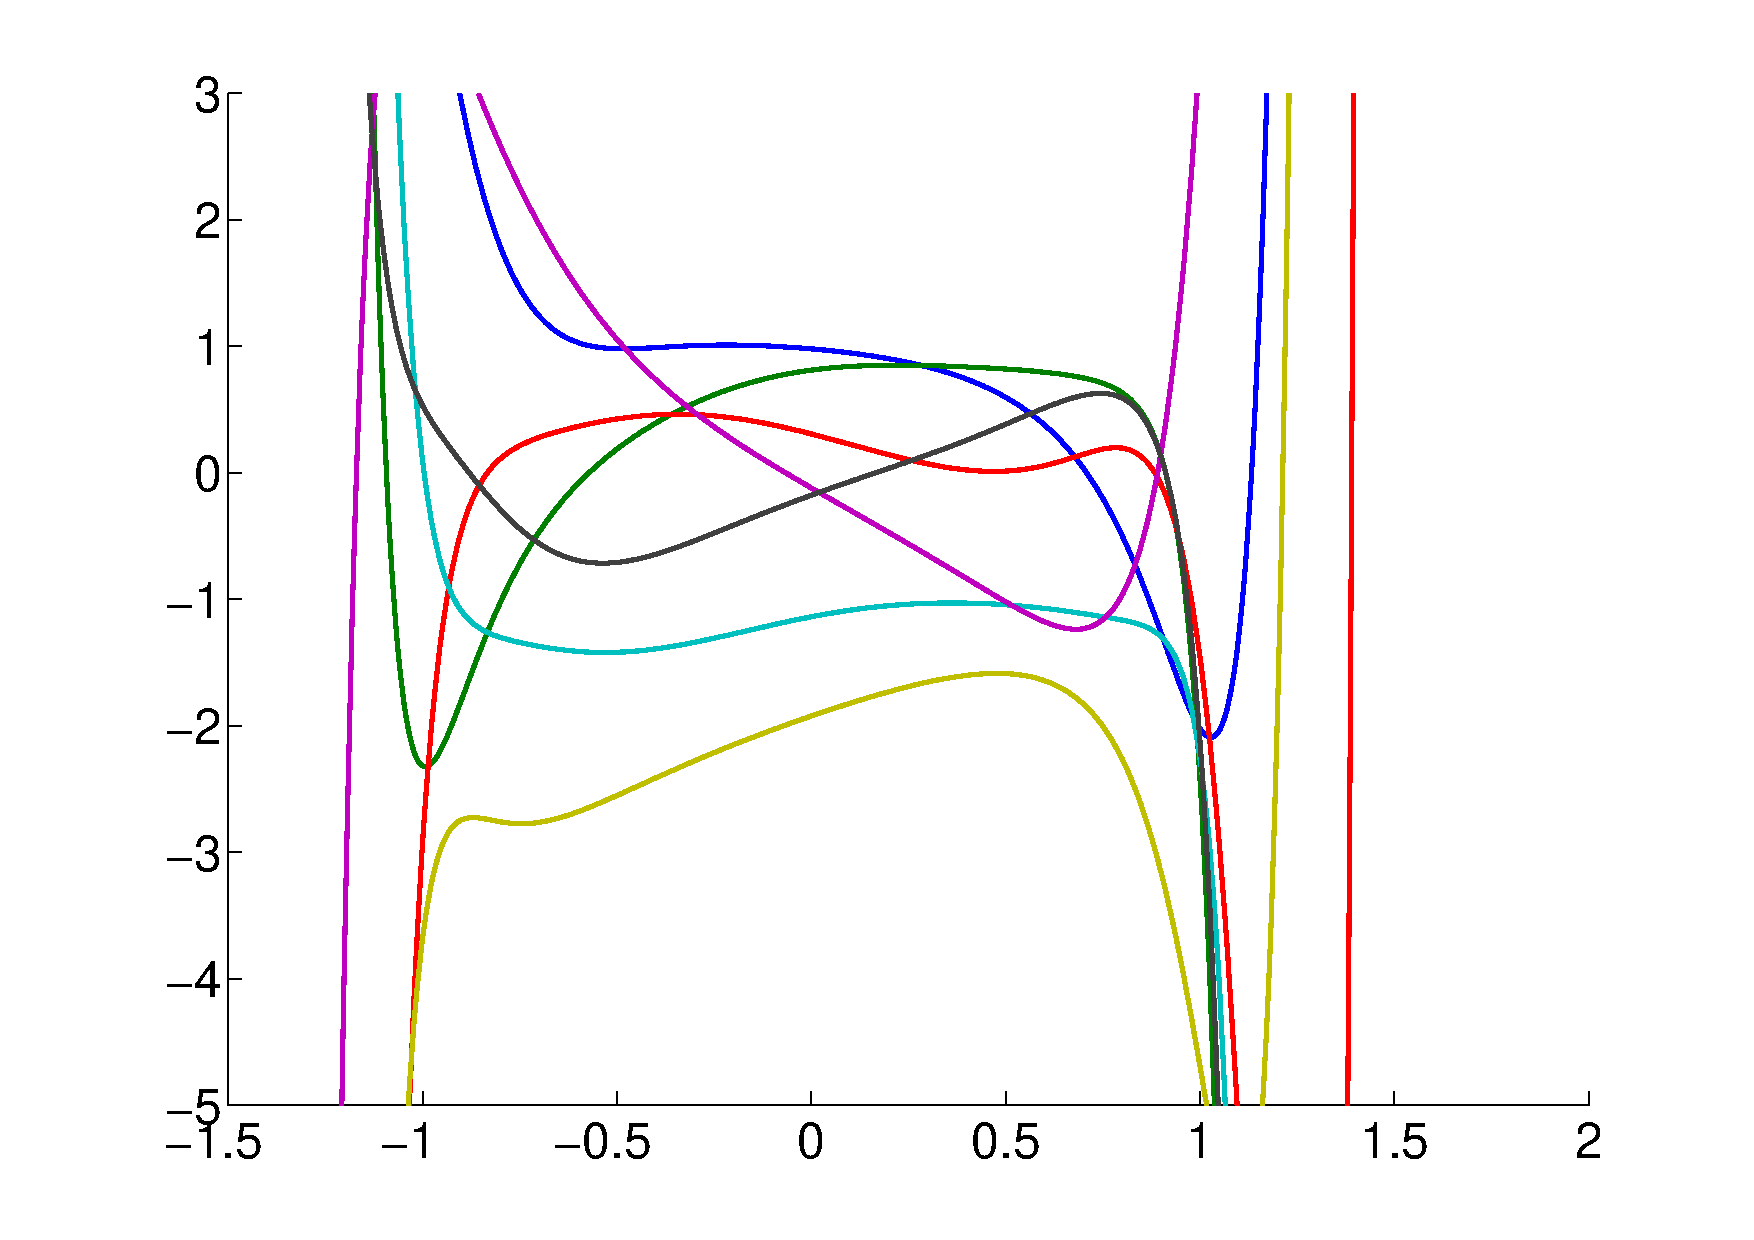
\includegraphics[width=0.45\textwidth]{random_polynomials_degree17.pdf}}
\centerline{Some samples from the prior}
}
\parbox{0.45\textwidth}{
\centerline{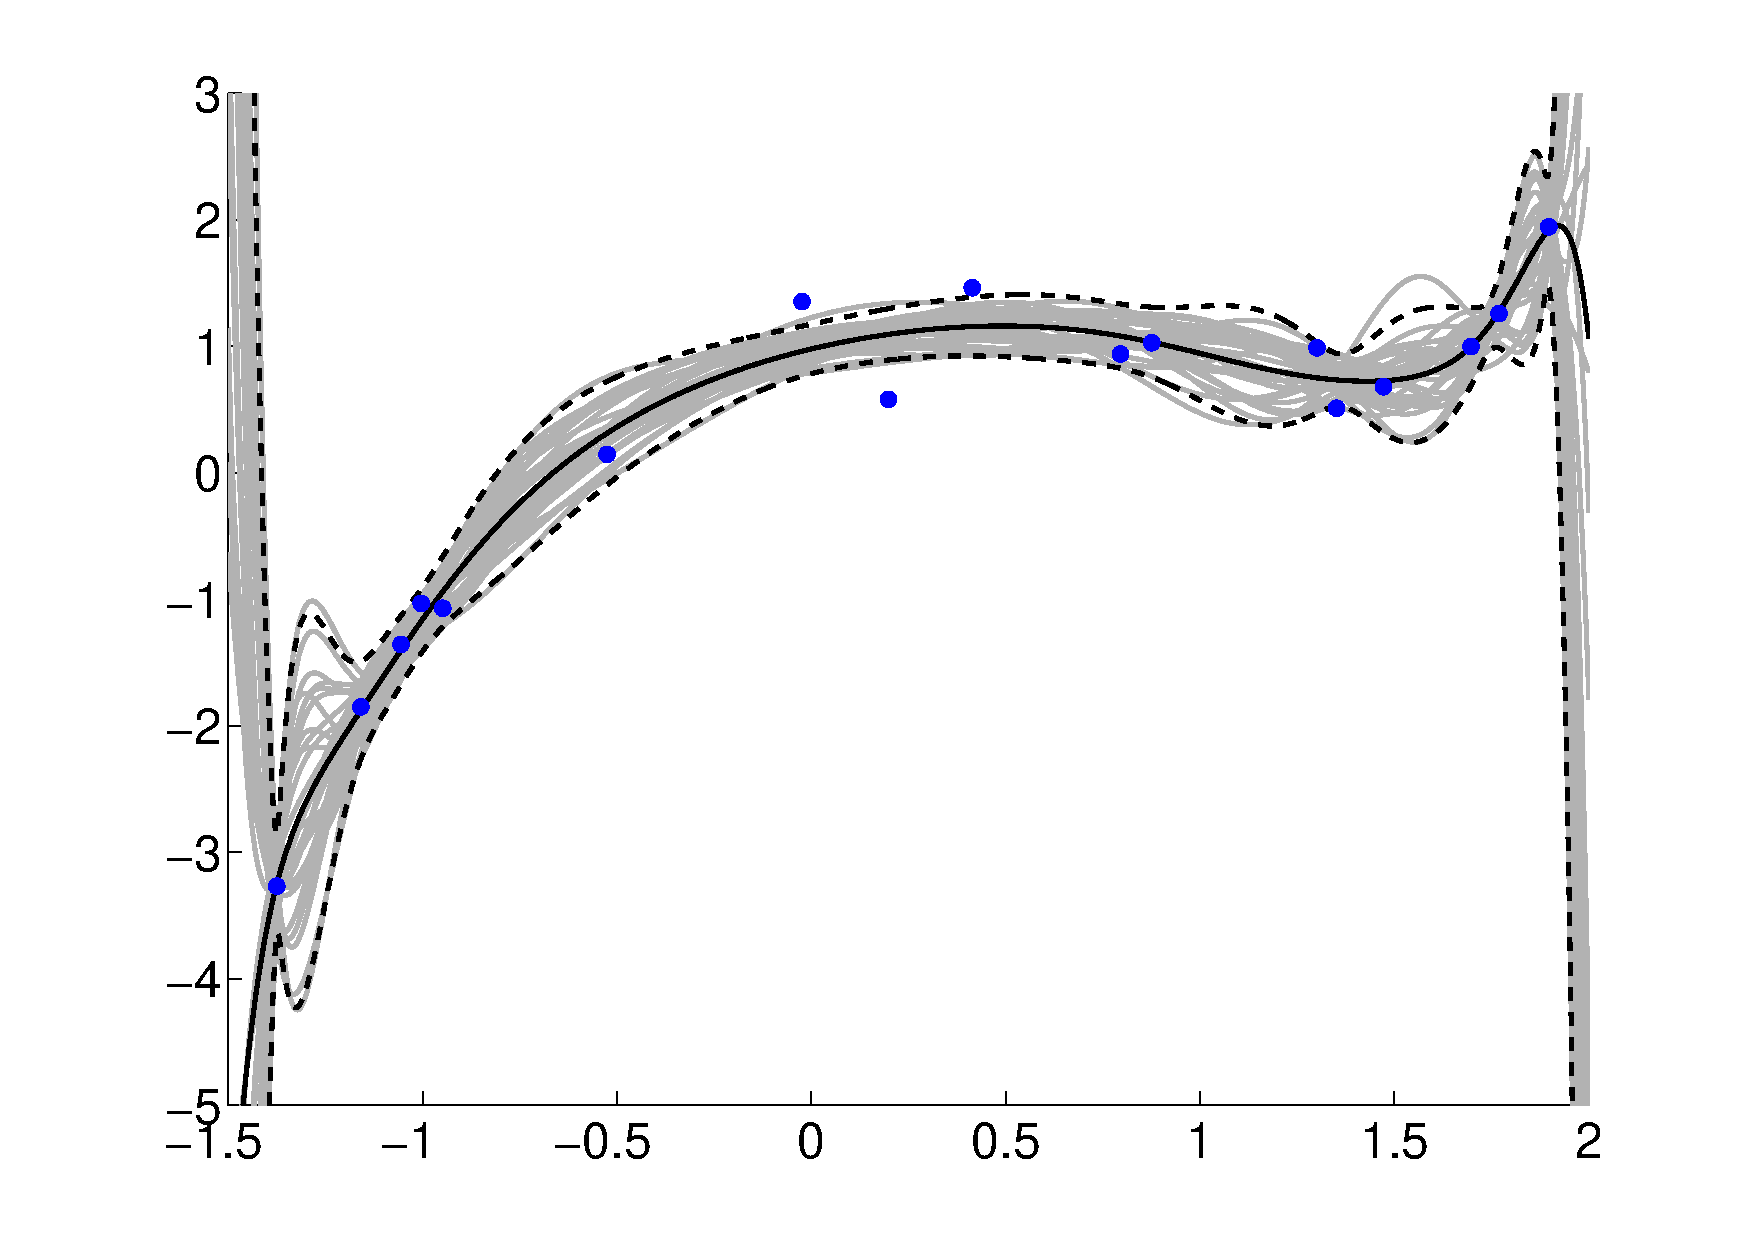
\includegraphics[width=0.45\textwidth]{samples_posterior_degree17.pdf}}
\centerline{Samples from the posterior}
}
\end{frame}


\begin{frame}
\frametitle{Are polynomials a good prior over functions?}

\centerline{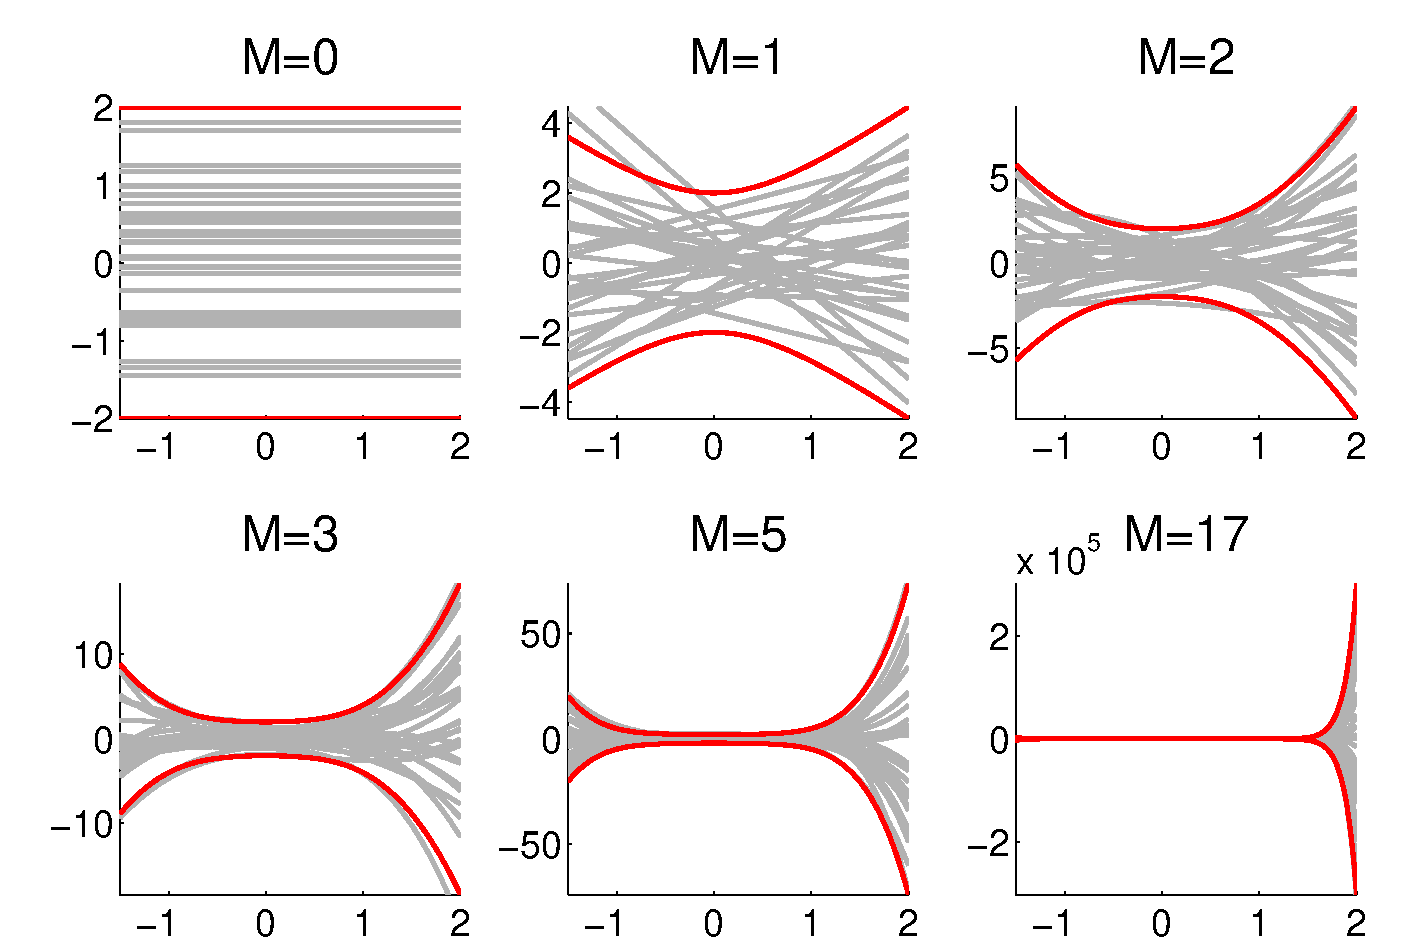
\includegraphics[width=\textwidth]{polynomial_prior_envelope}}
\end{frame}

\begin{frame}
\frametitle{A prior over functions view}

\centerline{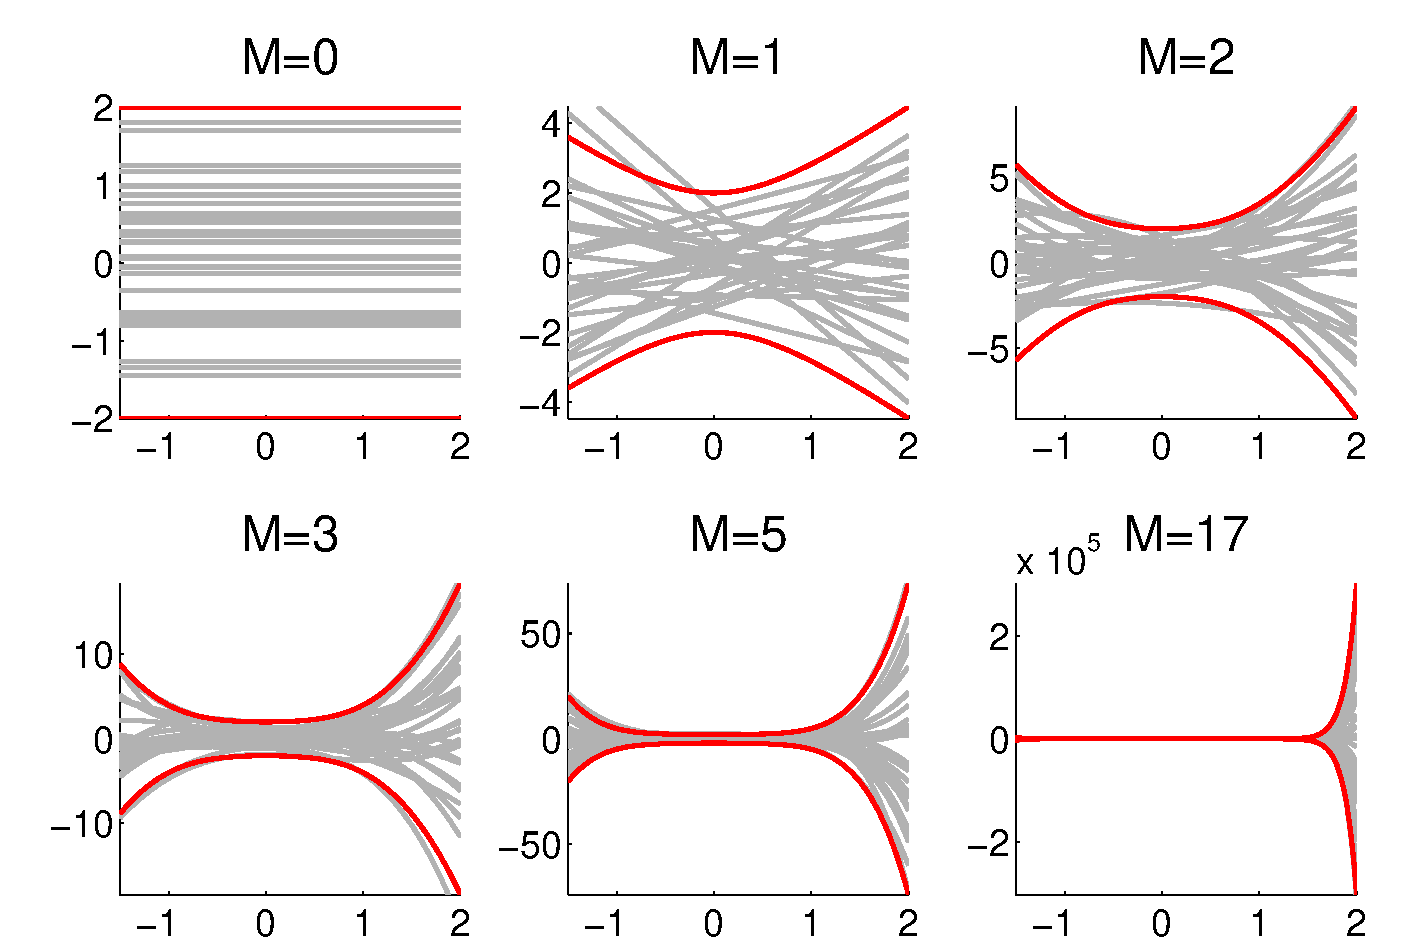
\includegraphics[width=0.35\textwidth]{polynomial_prior_envelope}}
%
We have learnt that linear-in-the-parameter models with priors on the weights
\Red{\emph{indirectly}} specify priors over functions.\\
\hfill\Blue{True... but those priors over functions might not be good.}\\
\vfill
\centerline{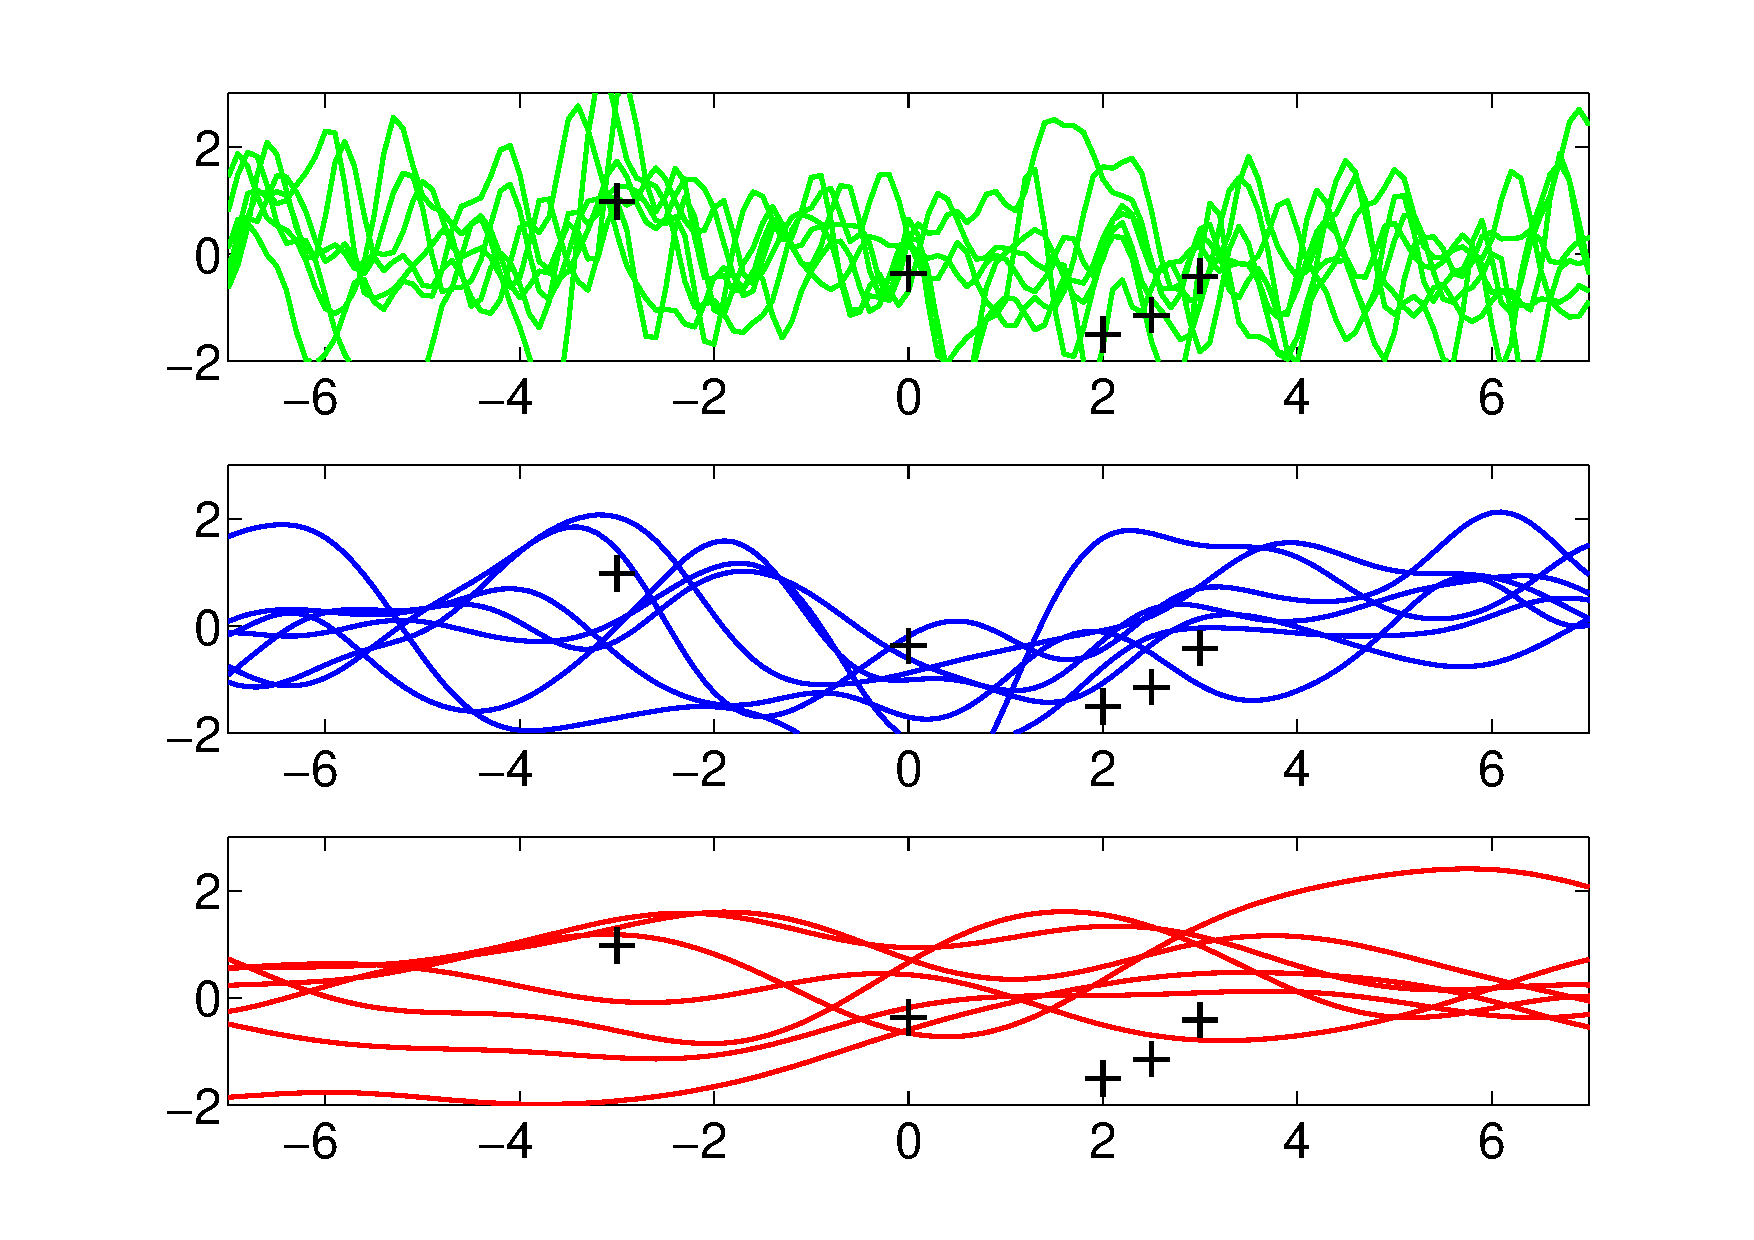
\includegraphics[width=0.35\textwidth]{rejection_sampling_data_priors.pdf}}
%
... why not try to specify priors over functions \Red{\emph{directly}}?\\
\hfill\Blue{What? What does a probability density over functions even look like?}
\end{frame}


\end{document}